% Universal Bootstrapping and Seeded Self-Hosting
% Publication-quality paper (Part 6)
%
% References to Lean formalization: lean/Cred/SeededSystem.lean,
% lean/Cred/MetaBootstrap.lean, lean/Cred/Commitment.lean, lean/Cred/ToyModel.lean,
% lean/Cred/Reflection.lean, lean/Cred/ReflectionTower.lean

\documentclass[11pt,a4paper]{article}

\usepackage{amsmath,amssymb,amsthm}
\usepackage{mathtools}
\usepackage{enumitem}
\usepackage{booktabs}
\usepackage{caption}
\usepackage{hyperref}
\hypersetup{
    colorlinks=true,
    linkcolor=blue,
    citecolor=blue,
    urlcolor=blue,
    pdfauthor={Christopher Albert},
    pdftitle={Universal Bootstrapping and Seeded Self-Hosting}
}
\usepackage{cleveref}
\usepackage[margin=1in]{geometry}
\emergencystretch=3em
\usepackage{tikz}
\usetikzlibrary{arrows.meta,positioning,shapes}
\usepackage{graphicx}

% Theorem environments
\newtheorem{theorem}{Theorem}[section]
\newtheorem{lemma}[theorem]{Lemma}
\newtheorem{proposition}[theorem]{Proposition}
\newtheorem{corollary}[theorem]{Corollary}
\newtheorem{definition}[theorem]{Definition}
\newtheorem{example}[theorem]{Example}
\newtheorem{remark}[theorem]{Remark}

% Custom commands
\newcommand{\cred}{\mathsf{cred}}
\newcommand{\negc}{\mathord{\sim}}
\newcommand{\conjc}{\otimes}
\newcommand{\disjc}{\sqcup}
\newcommand{\Cond}{\mathsf{Cond}}
\newcommand{\Real}{\mathbb{R}}
\newcommand{\Nat}{\mathbb{N}}
\newcommand{\Seed}{\mathrm{Seed}}
\newcommand{\SelfHosts}{\mathrm{SelfHosts}}
\newcommand{\run}{\mathrm{run}}

\title{Universal Bootstrapping and Seeded Self-Hosting}

\author{Christopher Albert\\
\small Institute for Theoretical and Computational Physics\\
\small Graz University of Technology}
\date{June 2026}

\begin{document}

\maketitle

\begin{abstract}
We give a formal account of bootstrapping: the pattern by which a system
produces a copy of itself from an artifact that an earlier copy produced.
We define a \emph{seeded system} as a tuple
$(S, \Seed, T, V, E)$ of a state space, a seed predicate, a transition,
a step validator, and a correctness relation, with the run
$\run\,s_0\,n = T^{[n]}\,s_0$ obtained by iterating $T$ from a seed.
Three theorems form the spine.
\emph{No empty bootstrap}: if no state satisfies $\Seed$, no state is a seed,
so no run begins.
\emph{Self-hosting from fixed points}: an $E$-fixed point of $T$ satisfies
$E\,s\,(T\,s)$ and is stationary.
\emph{Commitment conservation}: folding a substrate parameter $b$ into the
state leaves the observable orbit unchanged,
$(\mathrm{withSubstrate}\,T)^{[n]}(b,s) = (b, (T\,b)^{[n]}\,s)$,
so seed minimization is substrate-relative.
We instantiate the schema in the irreducible-commitment system and in a
stratified reflection tower, where the checker is sound at every level
$n+1$ for level $n$ but never closes at its own level, the constructive
shadow of the G\"odel/Tarski boundary.
All results are machine-checked in Lean~4 with Mathlib.
The schema is elementary audit discipline, not a deep theorem; cross-domain
readings are marked as remarks.
\end{abstract}

%=============================================================================
\section{Introduction}
\label{sec:intro}
%=============================================================================

A C compiler is itself a C program, so to build it one needs a C compiler.
The circle does not close in a vacuum: an earlier binary, produced outside the
present source, compiled the first version, and every later binary was built by
its predecessor~\cite{thompson1984}.
Strip the example to its parts and a fixed skeleton remains:
a space of artifacts, a \emph{seed} supplied from outside, a \emph{transition}
that builds the next artifact, a \emph{validator} on each step, and a notion of
when two artifacts count as the same.
The states where the transition reproduces its input \emph{self-host}.

This paper formalizes that skeleton and proves the small set of facts it
supports.
The formal object is the Lean structure \texttt{SeededSystem}, a tuple
$(S, \Seed, T, V, E)$ with the run defined by iterating $T$ from a seed.
Three results are the spine.
\emph{No empty bootstrap} (\Cref{thm:no-empty}): with no admissible seed there
is nothing to iterate.
\emph{Self-hosting from fixed points} (\Cref{thm:selfhost-fixed}): a fixed point
of $T$ that is $E$-related to itself self-hosts and is stationary.
\emph{Commitment conservation} (\Cref{thm:conservation}): relocating a substrate
parameter into the state leaves the orbit unchanged, so a small explicit seed is
small only relative to a fixed substrate.

The schema has instances.
The irreducible-commitment system of Part~4 embeds, with both its convergence
fixed point and its degenerate absorbing element self-hosting
(\Cref{thm:commit-embed,thm:commit-selfhost}).
A reflection tower indexed by $\Nat$ certifies a proof checker at every level:
level $n+1$ asserts the soundness of the level-$n$ checker, the step is always
available, and no level certifies itself
(\Cref{thm:tower,thm:self-boundary}).
That gap is the constructive shadow of G\"odel's second theorem and Tarski's
undefinability of truth~\cite{godel1931}.

\textbf{Positioning.}
The bootstrap theorems are elementary.
\Cref{thm:no-empty} is near-trivial as logic;
\Cref{thm:selfhost-fixed} is a rewrite;
\Cref{thm:conservation} is an induction.
Their value is as accounting discipline, not as deep mathematics: the schema
refuses to hide where the starting datum lives.
The cross-domain readings (compiler bootstrapping, proof kernels, origins of
order) are structured analogies, confined to remarks, and never asserted as
consequences of the theorems.
\Cref{tab:claim-hierarchy} separates the layers.
Each Lean name is cited once as ``(machine-checked, \texttt{name})''.

\textbf{Outline.}
\Cref{sec:schema} defines the seeded system and proves the spine.
\Cref{sec:commitment} embeds the commitment system.
\Cref{sec:conservation} proves commitment conservation.
\Cref{sec:reflection} builds the reflection tower and locates the
self-soundness boundary.
\Cref{sec:positioning} states the claim hierarchy.
Appendix~\ref{app:lean} records the formalization.

%=============================================================================
\section{The Seeded System}
\label{sec:schema}
%=============================================================================

This section defines the formal object and proves the three facts that depend
on nothing else.

\subsection{The schema}

\begin{definition}[Seeded system]
\label{def:seeded}
A \emph{seeded system} is a tuple $M = (S, \Seed, T, V, E)$ where
$S$ is a type of states,
$\Seed : S \to \mathrm{Prop}$ marks the admissible seeds,
$T : S \to S$ is the transition,
$V : S \to S \to \mathrm{Prop}$ is the step validator, and
$E : S \to S \to \mathrm{Prop}$ is the correctness relation.
\end{definition}

The five fields name the object ($S$), the operation ($T$), the constraint
($V$ and $\Seed$), and the consequence tracked ($E$).
In Lean this is the structure \texttt{SeededSystem} with fields \texttt{S},
\texttt{Seed}, \texttt{T}, \texttt{V}, \texttt{E}
(machine-checked, \texttt{SeededSystem}).

\begin{definition}[Run]
\label{def:run}
The \emph{run} of $M$ of length $n \in \Nat$ from a state $s_0 \in S$ is
\[
  \run\,s_0\,n := T^{[n]}\,s_0,
\]
the $n$-fold iterate of $T$ applied to $s_0$.
It satisfies $\run\,s_0\,0 = s_0$ and
$\run\,s_0\,(n+1) = T(\run\,s_0\,n)$.
\end{definition}

The unfolding identities are \texttt{run\_zero} and \texttt{run\_succ}
(machine-checked, \texttt{SeededSystem.run\_succ}).

\begin{figure}[t]
\centering
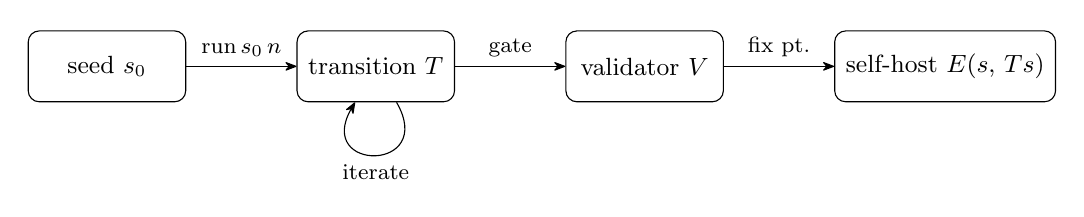
\begin{tikzpicture}[>={Stealth[round]},
  box/.style={draw, rounded corners, font=\small, minimum height=9mm,
    minimum width=20mm, inner sep=4pt}]
  \node[box] (seed) {seed $s_0$};
  \node[box, right=14mm of seed] (T) {transition $T$};
  \node[box, right=14mm of T] (V) {validator $V$};
  \node[box, right=14mm of V] (sh) {self-host $E(s,\,T s)$};
  \draw[->] (seed) -- node[above, font=\footnotesize] {$\run\,s_0\,n$} (T);
  \draw[->] (T) -- node[above, font=\footnotesize] {gate} (V);
  \draw[->] (V) -- node[above, font=\footnotesize] {fix pt.} (sh);
  \draw[->] (T) to[out=-60,in=-120,looseness=5] node[below, font=\footnotesize] {iterate} (T);
\end{tikzpicture}
\caption{The seeded system $(S, \Seed, T, V, E)$ of \Cref{def:seeded}.
A run iterates $T$ from a seed $s_0$ (\Cref{def:run}); the validator $V$ gates
each step; a self-hosting state satisfies $E(s, T s)$ (\Cref{def:selfhost}).
With no admissible seed the pipeline has no input (\Cref{thm:no-empty}).}
\label{fig:schema}
\end{figure}

A run needs a seed to iterate from.
The schema makes that literal.

\begin{theorem}[No empty bootstrap]
\label{thm:no-empty}
If $\neg\,\exists s,\ \Seed\,s$, then $\forall s,\ \neg\,\Seed\,s$.
\end{theorem}

\begin{proof}
Fix $s$ and assume $\Seed\,s$.
Then $\exists s,\ \Seed\,s$, contradicting the hypothesis.
Hence $\neg\,\Seed\,s$ for every $s$
(machine-checked, \texttt{SeededSystem.no\_empty\_bootstrap}).
\end{proof}

\begin{remark}[Where the datum lives]
\label{rem:no-empty}
\Cref{thm:no-empty} is trivial as logic, and that is the content.
A bootstrap never starts from nothing.
The information not supplied as a seed has not vanished; it has moved into the
substrate folded into $T$.
The theorem names the place that information must occupy without saying what
fills it.
\end{remark}

\subsection{Self-hosting}

\begin{definition}[Self-hosting]
\label{def:selfhost}
A state $s \in S$ \emph{self-hosts} when the transition reproduces it up to
correctness:
\[
  \SelfHosts\,s := E\,s\,(T\,s).
\]
\end{definition}

In Lean this is \texttt{SeededSystem.SelfHosts}
(machine-checked, \texttt{SeededSystem.SelfHosts}).
The simplest route to self-hosting is a fixed point.

\begin{theorem}[Self-hosting from fixed points]
\label{thm:selfhost-fixed}
Let $s \in S$.
If $E\,s\,s$ and $T\,s = s$, then $\SelfHosts\,s$.
\end{theorem}

\begin{proof}
The goal is $E\,s\,(T\,s)$.
Rewrite $T\,s$ to $s$ using $T\,s = s$; the goal becomes $E\,s\,s$, supplied by
hypothesis
(machine-checked, \texttt{SeededSystem.selfHosts\_of\_fixed}).
\end{proof}

\begin{proposition}[Fixed points are stationary]
\label{prop:stationary}
If $T\,s = s$, then $\run\,s\,n = s$ for every $n \in \Nat$.
\end{proposition}

\begin{proof}
Induction on $n$.
For $n = 0$, $\run\,s\,0 = s$ by \Cref{def:run}.
For the step, $\run\,s\,(n+1) = T(\run\,s\,n) = T\,s = s$ by the induction
hypothesis and $T\,s = s$
(machine-checked, \texttt{SeededSystem.run\_const\_of\_fixed}).
\end{proof}

The schema is inhabited.
The one-state system \texttt{trivialSelfHost} (state \texttt{Unit}, identity
transition, equality as $E$) has a self-hosting state by reflexivity, so
$\SelfHosts$ is not vacuous
(machine-checked, \texttt{trivialSelfHost\_selfHosts}).

\begin{remark}[The compiler reading]
\label{rem:compiler}
Read $T\,s$ as $\mathrm{compile}(s)$ and $E$ as observational equivalence.
Then $\SelfHosts\,s$ says the compiler recompiles to itself.
The two bootstrap strategies in practice instantiate the same five slots:
a large inherited toolchain seed builds the next compiler under a three-stage
rebuild validator~\cite{thompson1984}; a minimal audited path starts from a
few hundred bytes of hand-written hex and climbs by individually inspectable
stages~\cite{stage0,bootstrappable}.
Wheeler's diverse double-compiling~\cite{wheeler2005} is the validator $V$
doing work $E$ alone cannot: it checks reproduction against a diverse witness,
so a backdoor that survives self-comparison must also survive comparison with
an independent builder.
These readings illustrate \Cref{def:selfhost}; they are not proved by it.
\end{remark}

%=============================================================================
\section{The Commitment System as a Seeded System}
\label{sec:commitment}
%=============================================================================

Part~4 studied an irreducible-commitment structure on credences: a refinement
operator with a fixed point reached from every seed and a degenerate absorbing
element.
That structure is the metric instance of the schema, and the embedding is a
theorem.

\begin{definition}[Commitment system]
\label{def:commitment}
A \emph{commitment system} is a tuple $C = (op, fp, deg)$ with a refinement
operator $op : \mathrm{Credence} \to \mathrm{Credence}$, a fixed point
$fp$ with $op\,fp = fp$, and a degenerate element $deg$ with $op\,deg = deg$,
such that the orbit depends on the seed and converges to $fp$ from every seed.
\end{definition}

In Lean this is \texttt{Credence.CommitmentSystem}, carrying the four
properties \texttt{fixedPoint}, \texttt{seedMatters}, \texttt{converges}, and
\texttt{degAbsorbing} as fields
(machine-checked, \texttt{Credence.CommitmentSystem}).
The averaging contractions \texttt{commitmentToyHalf} and
\texttt{commitmentToyOne} are genuine instances with distinct fixed points.

\begin{theorem}[Commitment systems are seeded systems]
\label{thm:commit-embed}
Every commitment system $C$ yields a seeded system $C.\mathtt{toSeeded}$ with
state space $S = \mathrm{Credence}$, transition $T = C.op$, correctness
$E = {=}$, and every credence an admissible seed.
\end{theorem}

\begin{proof}
Define the fields of \Cref{def:seeded} from $C$: take $\Seed$ identically true,
$T = C.op$, $V$ identically true, and $E$ equality.
This is well typed, so it is a seeded system
(machine-checked, \texttt{Credence.CommitmentSystem.toSeeded}).
\end{proof}

\begin{theorem}[Fixed point and degenerate element self-host]
\label{thm:commit-selfhost}
For every commitment system $C$, both $C.fp$ and $C.deg$ self-host in
$C.\mathtt{toSeeded}$.
\end{theorem}

\begin{proof}
Apply \Cref{thm:selfhost-fixed}.
Correctness is equality, so $E\,s\,s$ holds by reflexivity for any $s$.
The transition is $C.op$, so $T\,C.fp = C.fp$ is the fixed-point equation
$op\,fp = fp$ and $T\,C.deg = C.deg$ is the absorption equation
$op\,deg = deg$
(machine-checked, \texttt{Credence.CommitmentSystem.fp\_selfHosts}).
The degenerate case is \texttt{deg\_selfHosts}.
\end{proof}

\begin{remark}[Two reasons to self-host]
\label{rem:two-reasons}
The two states self-host for opposite reasons.
The fixed point is the value the orbit certifies from any seed: the converged
commitment that reproduces itself.
The degenerate element is the absorbing zero of Cromwell's rule, unrecoverable
once entered, which reproduces itself by going nowhere.
The schema records both as $E\,s\,(T\,s)$.
In this embedding $V$ and $\Seed$ are trivial; a richer instance is where they
would separate a legitimate fixed point from a stuck one.
\end{remark}

%=============================================================================
\section{Commitment Conservation}
\label{sec:conservation}
%=============================================================================

Because $T$ folds the substrate in, shrinking the explicit seed need not shrink
the commitment: it can move into the substrate.
The following theorem makes the relocation exact.

\begin{definition}[Substrate-folded transition]
\label{def:withsubstrate}
Let $B$ and $S$ be types and $T : B \to S \to S$ a substrate-parameterized
transition.
The \emph{substrate-folded transition} on $B \times S$ is
\[
  \mathrm{withSubstrate}\,T := \lambda\,(b, s).\,(b,\ T\,b\,s),
\]
which carries the substrate $b$ in the state and evolves $s$ by $T\,b$.
\end{definition}

In Lean this is \texttt{withSubstrate}
(machine-checked, \texttt{withSubstrate}).

\begin{figure}[t]
\centering
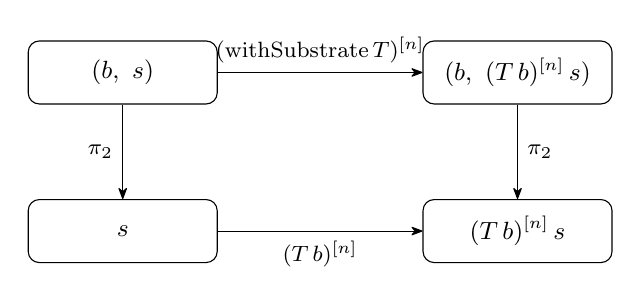
\begin{tikzpicture}[>={Stealth[round]},
  box/.style={draw, rounded corners, font=\small, minimum height=8mm,
    minimum width=24mm, inner sep=3pt}]
  \node[box] (bs0) {$(b,\ s)$};
  \node[box, right=26mm of bs0] (bs1) {$(b,\ (T\,b)^{[n]}\,s)$};
  \node[box, below=12mm of bs0] (s0) {$s$};
  \node[box, below=12mm of bs1] (s1) {$(T\,b)^{[n]}\,s$};
  \draw[->] (bs0) -- node[above, font=\footnotesize]
    {$(\mathrm{withSubstrate}\,T)^{[n]}$} (bs1);
  \draw[->] (s0) -- node[below, font=\footnotesize] {$(T\,b)^{[n]}$} (s1);
  \draw[->] (bs0) -- node[left, font=\footnotesize] {$\pi_2$} (s0);
  \draw[->] (bs1) -- node[right, font=\footnotesize] {$\pi_2$} (s1);
\end{tikzpicture}
\caption{Commitment conservation (\Cref{thm:conservation}).
Iterating the substrate-folded transition (top) and projecting to the second
component equals iterating $T\,b$ on $s$ directly (bottom).
The square commutes: the substrate $b$ is conserved in the state, the
observable orbit is unchanged. Relocating $b$ from transition parameter to seed
moves the commitment without removing it.}
\label{fig:conservation}
\end{figure}

\begin{theorem}[Commitment conservation]
\label{thm:conservation}
Let $T : B \to S \to S$, $b \in B$, $s \in S$.
For every $n \in \Nat$,
\[
  (\mathrm{withSubstrate}\,T)^{[n]}(b, s) = (b,\ (T\,b)^{[n]}\,s).
\]
\end{theorem}

\begin{proof}
Induction on $n$.
For $n = 0$ both sides are $(b, s)$.
For the step, expand the outer iterate once on each side.
The left side becomes
$(\mathrm{withSubstrate}\,T)\big((\mathrm{withSubstrate}\,T)^{[n]}(b,s)\big)$,
which by the induction hypothesis equals
$(\mathrm{withSubstrate}\,T)\,(b, (T\,b)^{[n]}\,s)
 = (b,\ T\,b\,((T\,b)^{[n]}\,s))$.
The right side becomes $(b,\ (T\,b)^{[n+1]}\,s)
 = (b,\ T\,b\,((T\,b)^{[n]}\,s))$.
The two sides agree
(machine-checked, \texttt{commitment\_conservation}).
\end{proof}

\begin{corollary}[Run invariance under relocation]
\label{cor:relocation}
Under the hypotheses of \Cref{thm:conservation}, the observable orbit is
unchanged by relocation:
$\big((\mathrm{withSubstrate}\,T)^{[n]}(b, s)\big)_2 = (T\,b)^{[n]}\,s$.
\end{corollary}

\begin{proof}
Project the equation of \Cref{thm:conservation} onto the second component
(machine-checked, \texttt{run\_invariant\_under\_relocation}).
\end{proof}

\begin{remark}[Seed minimization is substrate-relative]
\label{rem:minimization}
\Cref{thm:conservation} states that what is conserved is the pair
(substrate, seed), not the size of the explicit seed alone.
Carry the substrate $b$ in the state and the explicit seed grows to include $b$
while the substrate shrinks to nothing, yet nothing observable moves.
So every claim of a minimal seed is relative to a fixed substrate.
A Stage0 hex seed is small only against a fixed instruction set and loader;
a minimal proof kernel is small only against a fixed syntax, semantics, and
metatheory; a Solomonoff prior~\cite{solomonoff1964} is minimal in description
only against a chosen reference machine, which shifts every length by a
machine-dependent constant.
Maximum-entropy priors~\cite{jaynes2003} repeat the shape: the constraints held
fixed are the irreducible commitment the optimization does not supply.
Seed minimization sharpens the artifact and relocates the commitment; it does
not abolish it.
\end{remark}

%=============================================================================
\section{The Reflection Tower}
\label{sec:reflection}
%=============================================================================

The commitment embedding gives a single self-hosting fixed point.
Reflection gives a tower: level $n+1$ certifies level $n$, and no level
certifies itself.
The object certified is the foundation certificate checker
\texttt{checkFoundationCertificate} of Part~3, whose meta-level soundness
(\texttt{checkFoundationCertificate\_sound}) states that an accepted level-$n$
certificate denotes a genuine foundation consequence.

\begin{definition}[Reflection predicate]
\label{def:reflects}
A checked foundation proof \emph{reflects} the foundation threshold consequence
it stands for: $\mathrm{Reflects}(\mathit{checked})$ is the proposition
$\mathrm{FoundationThresholdConsequence}\ t\ \mathit{checked.premises}\
\mathit{checked.conclusion}$.
\end{definition}

In Lean this is \texttt{CheckedFoundationProof.Reflects}
(machine-checked, \texttt{CheckedFoundationProof.Reflects}).

\begin{proposition}[Acceptance reflects consequence]
\label{prop:reflects}
If $\mathrm{checkFoundationCertificate}\ t\ \mathit{tree} =
\mathrm{some}\ \mathit{checked}$, then $\mathrm{Reflects}(\mathit{checked})$.
\end{proposition}

\begin{proof}
The checker's soundness lemma applied to the acceptance hypothesis yields the
foundation consequence, which is exactly $\mathrm{Reflects}$ unfolded
(machine-checked, \texttt{checkFoundationCertificate\_reflects}).
\end{proof}

\Cref{prop:reflects} is one cross-level fact: Lean, acting as the level-$(n+1)$
verifier, certifies the level-$n$ checker.
The tower iterates it.

\begin{definition}[Level-indexed soundness]
\label{def:soundat}
For $n \in \Nat$ and a threshold $t$, $\mathrm{CheckerSoundAt}\ n\ t$ is the
proposition that every certificate tree the checker accepts at threshold $t$
yields its foundation consequence.
The index records the meta-standpoint, not the truth conditions.
\end{definition}

In Lean this is \texttt{CheckerSoundAt}
(machine-checked, \texttt{CheckerSoundAt}).

\begin{figure}[t]
\centering
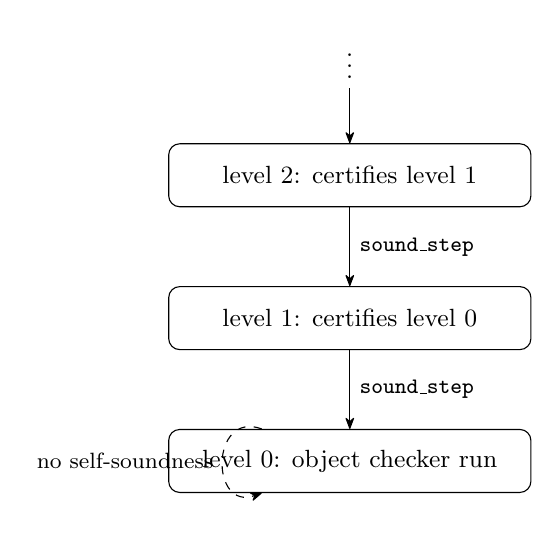
\begin{tikzpicture}[>={Stealth[round]},
  lvl/.style={draw, rounded corners, font=\small, minimum height=8mm,
    minimum width=46mm, inner sep=3pt}]
  \node[lvl] (l0) {level $0$: object checker run};
  \node[lvl, above=10mm of l0] (l1) {level $1$: certifies level $0$};
  \node[lvl, above=10mm of l1] (l2) {level $2$: certifies level $1$};
  \node[above=7mm of l2, font=\small] (dots) {$\vdots$};
  \draw[->] (l1) -- node[right, font=\footnotesize] {\texttt{sound\_step}} (l0);
  \draw[->] (l2) -- node[right, font=\footnotesize] {\texttt{sound\_step}} (l1);
  \draw[->] (dots) -- (l2);
  \draw[->, dashed] (l0) to[out=160,in=200,looseness=2.2]
    node[left, font=\footnotesize] {no self-soundness} (l0);
\end{tikzpicture}
\caption{The reflection tower (\Cref{thm:tower}).
Each level $n+1$ certifies the soundness of the level-$n$ checker by
\texttt{sound\_step}; \texttt{checker\_sound\_at} populates every level by
induction. The dashed self-loop is the gap the tower keeps open: no level
certifies itself at its own level (\Cref{thm:self-boundary}).}
\label{fig:tower}
\end{figure}

\begin{theorem}[Reflection tower]
\label{thm:tower}
For every $n \in \Nat$ and threshold $t$, $\mathrm{CheckerSoundAt}\ n\ t$ holds.
\end{theorem}

\begin{proof}
Induction on $n$.
The base $\mathrm{CheckerSoundAt}\ 0\ t$ is \Cref{prop:reflects} packaged at
index $0$ (\texttt{checker\_sound\_at\_zero}).
For the step, $\mathrm{CheckerSoundAt}\ (n+1)\ t$ follows by reapplying the same
meta-level reflection lemma; the level-$n$ hypothesis is not consumed, which is
the precise sense in which level $n+1$ certifies the level-$n$ checker
(\texttt{sound\_step})
(machine-checked, \texttt{checker\_sound\_at}).
\end{proof}

\begin{proposition}[Monotonicity]
\label{prop:tower-mono}
If $n \le m$ and $\mathrm{CheckerSoundAt}\ n\ t$ holds, then
$\mathrm{CheckerSoundAt}\ m\ t$ holds.
\end{proposition}

\begin{proof}
$\mathrm{CheckerSoundAt}\ m\ t$ holds for every $m$ by \Cref{thm:tower},
so it holds in particular at $m \ge n$
(machine-checked, \texttt{checker\_sound\_at\_mono}).
\end{proof}

\begin{theorem}[Self-soundness boundary]
\label{thm:self-boundary}
The strict step is always provable: for every $n$ and $t$,
\[
  \mathrm{CheckerSoundAt}\ n\ t \;\Rightarrow\;
  \mathrm{CheckerSoundAt}\ (n+1)\ t.
\]
The tower provides no term certifying $\mathrm{CheckerSoundAt}\ n\ t$ from
within level $n$ itself.
\end{theorem}

\begin{proof}
The implication is witnessed by \texttt{sound\_step}: from any standpoint at
level $n$, the meta-level reflection lemma re-establishes soundness at level
$n+1$
(machine-checked, \texttt{self\_soundness\_boundary}).
The step strictly raises the index; there is no content-adding
$\mathrm{CheckerSoundAt}\ n\ t \Rightarrow \mathrm{CheckerSoundAt}\ n\ t$ in
the development.
\end{proof}

\begin{remark}[The G\"odel/Tarski boundary]
\label{rem:godel}
\Cref{thm:self-boundary} is the constructive shadow of incompleteness.
A theory strong enough for arithmetic cannot prove its own consistency
\cite{godel1931}; it can adjoin the reflection principle ``if $T$ proves
$\varphi$ then $\varphi$'' to obtain a strictly stronger theory, and iterating
this transfinitely is Turing's ordinal logics~\cite{turing1939} and Feferman's
recursive progressions~\cite{feferman1962}.
Each adjoined soundness statement is again an arithmetic sentence, so the new
theory is again incomplete, and the tower only ever pushes the boundary up.
The reflection tower realizes the same stratification: \texttt{sound\_step}
always climbs one level, and the self-loop of \Cref{fig:tower} stays open.
A system can host itself operationally (\Cref{thm:selfhost-fixed}) but cannot
crisply certify itself at its own level.
\end{remark}

%=============================================================================
\section{Positioning and the Claim Hierarchy}
\label{sec:positioning}
%=============================================================================

The bootstrap theorems are deliberately elementary.
\Cref{thm:no-empty} (no seed, no run) is a contradiction;
\Cref{thm:selfhost-fixed} (fixed point gives self-hosting) is a rewrite;
\Cref{thm:conservation} (commitment conservation) is an induction.
Their role is an accounting discipline, like double-entry bookkeeping:
useful because it catches a hidden host tool in a trusted compiler path, a
hidden substrate in a Bayesian comparison, or a hidden validator assumption in
a self-hosting claim.
\Cref{tab:claim-hierarchy} separates the layers so the schema is not read as
carrying weight it does not.

\begin{table}[t]
\centering
\small
\begin{tabular}{@{}lll@{}}
\toprule
Claim & Status & Depth \\
\midrule
No seed, no run (\Cref{thm:no-empty}) & elementary theorem & bookkeeping \\
Fixed point gives self-hosting (\Cref{thm:selfhost-fixed})
  & elementary theorem & bookkeeping \\
Commitment conservation (\Cref{thm:conservation})
  & elementary theorem & bookkeeping \\
Commitment system embeds (\Cref{thm:commit-embed})
  & structural theorem & schema instance \\
Reflection tower (\Cref{thm:tower}) & inductive theorem & schema instance \\
Self-soundness boundary (\Cref{thm:self-boundary})
  & boundary theorem & incompleteness shadow \\
Compiler / kernel / origins readings & structured analogy & expository \\
\bottomrule
\end{tabular}
\caption{The claim hierarchy.
The bootstrap rows are elementary bookkeeping; the embedding and tower are
schema instances; the cross-domain readings are analogies confined to remarks.
The paper claims each row only at its stated depth.}
\label{tab:claim-hierarchy}
\end{table}

\begin{remark}[Cross-domain readings]
\label{rem:cross-domain}
The schema recurs as a description, not a unification theorem.
A proof kernel reads as substrate (elaborated terms), seed (a trusted checker),
transition (elaborate and check), and validator (an independent re-check, as in
Lean4Lean~\cite{carneiro2024}); the self-host condition is that the kernel
certifies its own exported proof.
Accounts of life's origin fill the same slots: an autocatalytic
set~\cite{kauffman1993} as seed, replication as transition, selection as
validator, with the hypercycle~\cite{eigen1971} and protocell
synthesis~\cite{szostak2001} as the concrete chemistry.
These readings are structured analogies.
The recurrence of one bookkeeping pattern is not a shared cause:
Anderson's point that more is different~\cite{anderson1972} cuts against any
claim that a single schema explains complexity, since new levels carry laws the
lower level does not contain.
The schema does not show that all complexity shares an origin, that biology is
designed, or that any system bootstraps from nothing.
\Cref{thm:no-empty} states the last in the negative: a seed is required.
\end{remark}

%=============================================================================
\section{Conclusion}
\label{sec:conclusion}
%=============================================================================

The seeded system $(S, \Seed, T, V, E)$ supports a small, exact spine.
No run begins without a seed (\Cref{thm:no-empty});
a fixed point of the transition self-hosts and is stationary
(\Cref{thm:selfhost-fixed,prop:stationary});
relocating a substrate parameter into the state conserves the observable orbit
(\Cref{thm:conservation}), so seed minimization is substrate-relative.
The schema is inhabited by the irreducible-commitment system, whose fixed point
and degenerate element both self-host
(\Cref{thm:commit-embed,thm:commit-selfhost}), and by a reflection tower that
certifies a proof checker at every level $n+1$ for level $n$ but never at its
own level (\Cref{thm:tower,thm:self-boundary}), the constructive shadow of the
G\"odel/Tarski boundary.
All results are machine-checked in Lean~4 with Mathlib (Appendix~\ref{app:lean}).
The schema is elementary audit discipline.
Its contribution is to make the seed explicit: every bootstrap names a seed, and
the work is to keep that seed minimal, stated, and open to audit, not to pretend
it can be zero.

\section*{Acknowledgements}

Anthropic's Claude was used as an assistant for both the Lean formalization and
the manuscript preparation.

%=============================================================================
% Bibliography
%=============================================================================

\bibliographystyle{plain}
\bibliography{../cred}

%=============================================================================
% APPENDIX
%=============================================================================
\appendix

%=============================================================================
\section{Lean Formalization}
\label{app:lean}
%=============================================================================

The results are formalized in Lean~4 with Mathlib.
The bootstrap schema and conservation are in \texttt{Cred/SeededSystem.lean} and
\texttt{Cred/MetaBootstrap.lean}; the commitment instance is in
\texttt{Cred/Commitment.lean} and \texttt{Cred/ToyModel.lean}; the reflection
tower is in \texttt{Cred/Reflection.lean} and \texttt{Cred/ReflectionTower.lean}.

\textbf{Key definitions.}

\medskip
\noindent
\texttt{structure SeededSystem where}\\
\null\quad \texttt{S : Type}\\
\null\quad \texttt{Seed : S}~$\to$~\texttt{Prop}\\
\null\quad \texttt{T : S}~$\to$~\texttt{S}\\
\null\quad \texttt{V : S}~$\to$~\texttt{S}~$\to$~\texttt{Prop}\\
\null\quad \texttt{E : S}~$\to$~\texttt{S}~$\to$~\texttt{Prop}

\medskip
\noindent
\texttt{def run (s0 : M.S) (n :}~$\Nat$\texttt{) : M.S := M.T\^{}[n] s0}

\medskip
\noindent
\texttt{def SelfHosts (s : M.S) : Prop := M.E s (M.T s)}

\medskip
\textbf{Key theorems.}
\begin{itemize}[nosep]
\item \texttt{no\_empty\_bootstrap}: no seed, no run
  (\Cref{thm:no-empty}).
\item \texttt{selfHosts\_of\_fixed}, \texttt{run\_const\_of\_fixed}:
  fixed-point self-hosting and stationarity
  (\Cref{thm:selfhost-fixed,prop:stationary}).
\item \texttt{trivialSelfHost\_selfHosts}: the schema is inhabited.
\item \texttt{Credence.CommitmentSystem.toSeeded}, \texttt{fp\_selfHosts},
  \texttt{deg\_selfHosts}: commitment embedding
  (\Cref{thm:commit-embed,thm:commit-selfhost}).
\item \texttt{commitment\_conservation},
  \texttt{run\_invariant\_under\_relocation}: conservation
  (\Cref{thm:conservation}, \Cref{cor:relocation}).
\item \texttt{checkFoundationCertificate\_reflects},
  \texttt{CheckerSoundAt}, \texttt{checker\_sound\_at},
  \texttt{checker\_sound\_at\_mono},
  \texttt{self\_soundness\_boundary}: the reflection tower
  (\Cref{prop:reflects,thm:tower,prop:tower-mono,thm:self-boundary}).
\end{itemize}

Verification: \texttt{cd lean \&\& lake build}.
Toolchain: Lean 4.16.0 with Mathlib 4.16.0.

\end{document}
